\section{Escalabilidade}

A escalabilidade da aplicação é sua capacidade de se adequar a um
amplo volume de requisições, mantendo a estabilidade do sistema e a
velocidade de respostas. Um sistema escalável está apto para responder
adequadamente nestes momentos, assim como liberar seus recursos em
momentos com poucas requisições.

Por se tratar de algo relativo ao processamento de requisições, a
escalabilidade diz respeito ao \gls{backend}, que centraliza os
pedidos dos usuários. A camada cliente por outro lado, por focar
exclusivamente na lógica de visualização, e rodar em dispositivos
mobile, não exige tanta capacidade de processamento, e a
escalabilidade não é uma preocupação para esta camada.

A ferramenta Jenkins, usada antes para a implantação da aplicação,
serve também como instrumento para gerenciar o número de instâncias em
produção. Por manter um histórico das versões ja usadas, a ferramenta
permite selecionar facilmente uma versão antiga caso seja necessária
uma ou mais instâncias novas em produção. O diagrama
\ref{fig:escalabilidade} demonstra como como este processo ocorre: a
partir de imagens salvas dos \gls{deploy} anteriores, uma nova
instância da aplicação é levantada para dividir a carga colocada entre
elas.

\begin{figure}
  \centering
  \caption{Diagrama de escalabilidade}
  \label{fig:escalabilidade}
  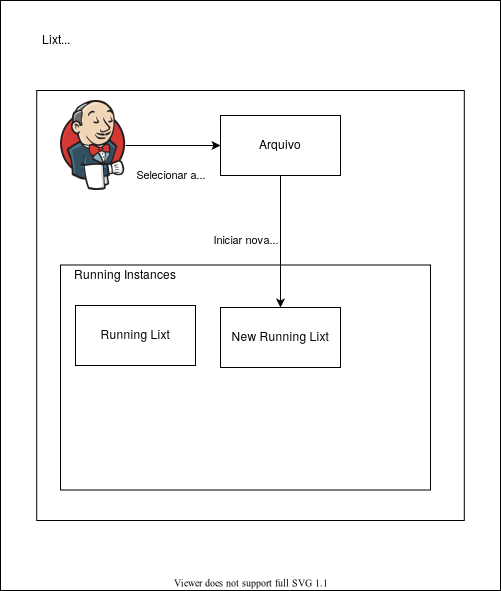
\includegraphics[scale=0.50]{images/escalar}
\end{figure}

Isto significa ainda que uma ferramenta de \gls{proxy} reverso é necessária
para realizar o \gls{load-balancing} entre as diversas instâncias que
compõe o \gls{backend}. Uma ferramenta deste tipo, como o Spring Cloud
Gateway, protege a aplicação, ao concentrar todas as requisições
externas, e em seguida, direcioná-las internamente entre as
instâncias, sem que o usuário final tenha acesso ao endereço delas e
portanto não possa fazer requisições diretamente a elas.
O diagrama \ref{fig:proxy} demontra o funcionamento deste proxy
reverso.

\begin{figure}
  \centering
  \caption{Funcionamento de um proxy reverso.}
  \label{fig:proxy}
  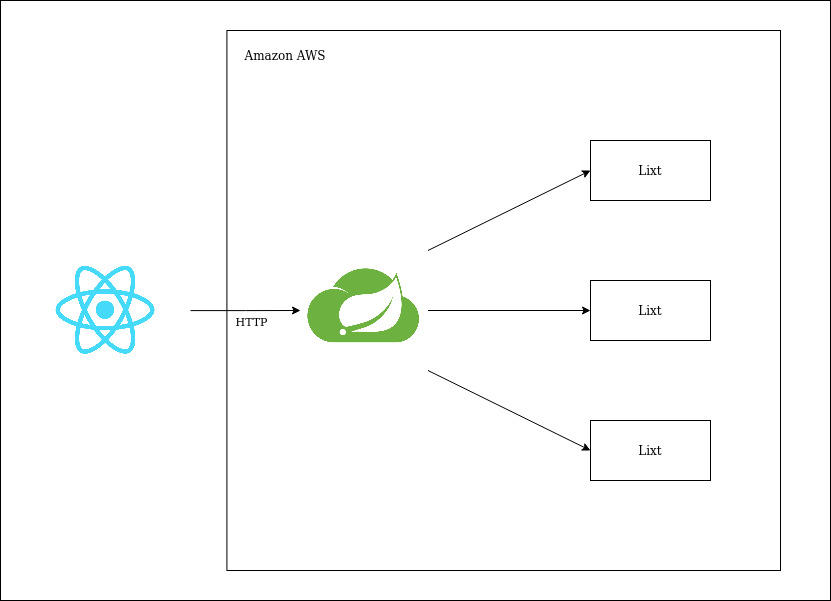
\includegraphics[scale=0.50]{proxy}
\end{figure}

Desta forma, uma instância de um proxy reverso deve estar rodando
enquanto a aplicação estiver rodando. A ferramenta Jenkins também será
usada para gerenciar esta aplicação, que deve ser menor e
relativamente mais simples em relação à aplicação principal do Lixt.

%%% Local Variables:
%%% mode: latex
%%% TeX-master: "../../main-texto-completo.tex"
%%% End:
